\documentclass[12pt]{jarticle}
\usepackage[dvipdfmx]{graphicx}
\usepackage{amsmath}

\setlength{\topmargin}{30mm}
\addtolength{\topmargin}{-1in}
\setlength{\oddsidemargin}{20mm}
\addtolength{\oddsidemargin}{-1in}
\setlength{\evensidemargin}{20mm}
\addtolength{\evensidemargin}{-1in}
\setlength{\textwidth}{170mm}
\setlength{\textheight}{245mm}
\setlength{\headsep}{0mm}
\setlength{\headheight}{0mm}
\setlength{\topskip}{0mm}



\begin{document}

\pagestyle{empty}
\begin{center}
  \vspace*{3.0cm}
  \underline{\bf{\fontsize{50pt}{100pt}\selectfont 卒業論文中間報告}}

  \vspace*{2.0cm}
  \begin{LARGE}
    Twitterを用いた新聞記事への\\
    自動ソーシャルアノテーションツールに関する研究
    \vspace*{2.0cm}

    平成 25 年 9 月 20 日提出
  \end{LARGE}

\end{center}
\begin{LARGE}
  \vspace*{1.0cm}
  \hspace{25mm}指導教員\hspace{51mm}伊庭斉志\,教授

  \hspace{70mm}ダヌシカ ボレガラ\,講師

  \vspace*{1.0cm}
  \begin{center}
    電子情報工学科

    \vspace{1.0cm}
    03-120443\hspace{15mm}村上\,晋太郎
  \end{center}

\end{LARGE}


\newpage
\tableofcontents

\newpage
\setcounter{page}{1}
\pagestyle{plain}

\section{序論}
\subsection{背景}
2000年代後半から、Facebook, Twitter, Google+などのソーシャルネットワーキングサービスが盛んに利用されるようになった。2012年には、Facebookのアクティブユーザ数は10億人\footnote{http://ja.wikipedia.org/wiki/Facebook}を突破し、Twitterでもアクティブユーザー数は1.4億人\footnote{http://www.724685.com/twitter/tw13050310.htm}となっている。Facebookでは一日当たり0.5ペタバイトのデータが増加しており、Twitterへの投稿数は一日当たり3.4億投稿となっている。
このように、ソーシャルネットワーキングサービスは利用者数の面でも、データ量の面でも莫大な資源となっており、様々な利用が期待される。

一方、近年インターネット上で閲覧することが出来るニュース記事が増加している。日本では、朝日新聞社\footnote{http://www.asahi.com}、読売新聞社\footnote{http://www.yomiuri.co.jp}、毎日新聞\footnote{http://mainichi.jp}等の大手新聞者がインターネット上でニュース記事を配信している。海外でも、Washington Post\footnote{http://www.washingtonpost.com} Las Angels Times\footnote{http://articles.latimes.com}等、大手新聞社が同様のサービスを提供している。

ソーシャルネットワーキングサービスの書き込みの中には、このようなインターネット上のニュース記事に言及しているものが多数存在する。このような書き込みには、一般のインターネットユーザーの個人的な意見、見解が記されている。このような、インターネット上のニュース記事とソーシャルネットワーキングサービスへの書き込みを結びつけることで、報道機関のプロの書き手と、ソーシャルネットワーキングサービス上の一般の書き手を結びつけることができるようになる。現在、ソーシャルネットワーキングサービスとインターネット上のニュースを関連づける研究として「(ここに先行研究を提示)」等が存在する。

\subsection{目的}
本研究では、ソーシャルネットワーキングサービス「Twitter」上の投稿(以下、「tweet」と記載する)をインターネット上のニュース記事に自動付与(アノテーション)するツールを作成することを目的とする。tweetの付与は、ニュース記事単位を付与の対象とするのではなく、ニュース記事の中の文単位を付与の対象とする(図\ref{fig1})。結果、ニュース中のどの部分に対して、Twitter上でどのような反応が起こっているのかが分かるようになる。このようなツールが実現すれば、ニュース記者にとってはは自分の書いた記事についてのユーザーの意見が簡単に見れるようになり、フィードバックをすぐに得る事ができるようになるという点で有用である。一方、読者にとっては、難しい内容のニュース記事でも他のユーザーによる情報付与があることにより、理解と助けとすることができる。

\begin{figure}[htbp]
  \begin{center}
    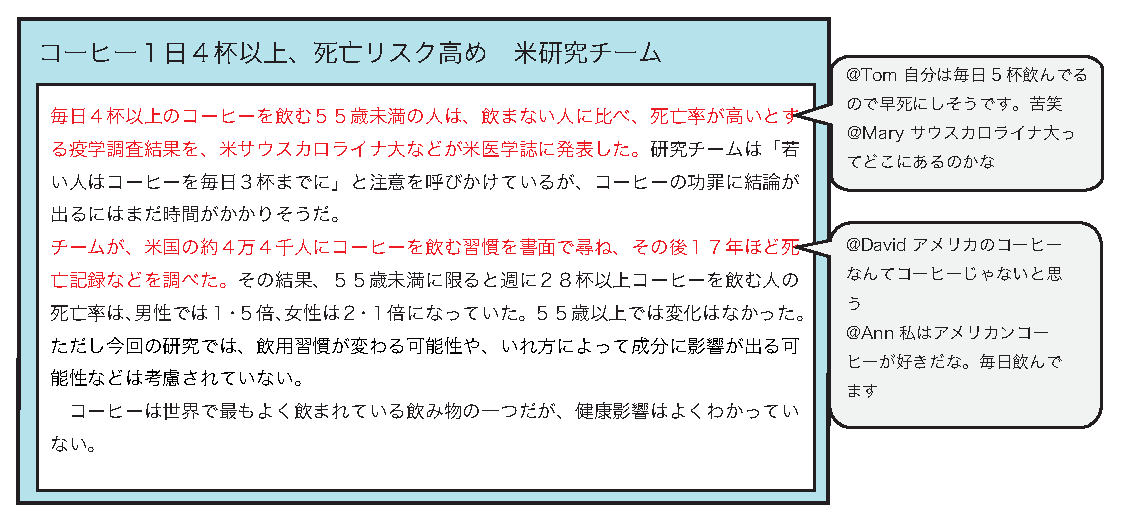
\includegraphics{ai/social_annotation.eps}
  \end{center}
  \caption{Twitterを用いたソーシャルアノテーションツール}
  \label{fig1}
\end{figure}

本研究ではTwitterとインターネット上のニュース記事を対象にツールの構築を進めていくが、その本質は「大きな文章中のセンテンスの集合と、小さな文章の集合のアラインメント」である。そのため、本研究で得られた成果は、Twitterやインターネット上のニュース記事に限らずに応用可能である。例えば、学術論文中の文に、その論文に対する意見、指摘、感想を自動付与するツールを作ることも可能である。

\section{手法}
本研究では、短文と短文を比較して、関連度の高いもの同士を結びつけるというタスクを行う。これをテキストアラインメントという。ここではその中で使用する手法について説明する。

\subsection{基本方針}
自然言語の文の特性を調べる際に、bag-of-words\cite{nlpml}という考え方がる。bag-of-wordsでは、ある文の特性を解析する際に、その文にどのような単語がどのくらい含まれているのかを計算して、それをもとに文の特性を解析し、クラスタリング等のタスクを行う。本研究でも、記事中のセンテンスに含まれる単語と、Tweetに含まれる単語の集合を比較して、記事中のセンテンスとTweetの関連度を計算する。

単語をもとに記事中のセンテンスとtweetの関連度を計算する際の指標として、以下の三つが挙げられる。

\begin{enumerate}
 \item 完全に一致する単語\\
    記事中のセンテンスとTweetの間に完全に一致する単語がある場合、そのセンテンスとTweetの関連度は高いと考えられる。図\ref{fig1}の例では、@Maryというユーザーが投稿したtweetに「サウスカロライナ」という単語が含まれているので、同じ単語を含む一つ目のセンテンスとの関連度が高くなる。
 \item 言い換えの単語\\
    記事中のセンテンスとtweetに言い換えの関係にある単語が含まれている場合、そのセンテンスとTweetの関連度は高くなると考えられる。図\ref{fig1}の例では、@Davidというユーザーが投稿したtweetに「米国」と言い換えの関係にある「アメリカ」という単語が含まれているので、「米国」という単語が含まれる、5行目から始まるセンテンスとの関連度が高くなる。
 \item 互いに類似する単語\\
    記事中のセンテンスとtweetの文に、同じ文脈で使われるような単語が含まれている場合、そのセンテンスとTweetの関連度は高くなると考えられる。図\ref{fig1}の例では、@Tomというユーザーが投稿したTweetに「早死に」という単語が含まれており、これは「死亡率」という単語と同じ文脈で使われる単語であると判断できるので、一行目から始まるセンテンスとの関連度が高くなる。
\end{enumerate}

これらの単語が含まれていたら、値が高くなるようにセンテンスとtweetの関連度を定義すれば、ニュース記事中のセンテンスとtweetのアラインメントをとることができる。

1.の「完全に一致する単語」は容易に発見することができる。それに対して、2.の「言い換えの単語」や、3.の「互いに類似する単語」を識別するためには、統計的な処理が必要となる。

また、1.の「完全に一致する単語」の中でも、「て」「に」「を」「は」等の助詞や助動詞等は、仮に記事中のセンテンスとtweetの間で一致したとしても両者の関連度には全く影響が無いと考えられる。同じように、「〜する」といった、それ自体が意味を持たない単語も一致したも関連度に影響しない。それに対して、「サウスカロライナ」のような固有名詞は一致した場合に関連度への影響が大きくなる。このような単語を「内容語」と言い、逆に助詞や助動詞、意味を持たない動詞などを「機能語」という。上記のそれぞれの指標から的確に関連度を計算するためには「内容語」の抽出が必要であり、そのためにも統計的な処理が必要となる。本研究ではtf-idf\cite{tfidf}という手法を使って内容語の抽出を行う。

\subsection{内容語の抽出}
上で述べたように、内容語の抽出にはtf-idf法\cite{tfidf}を使う。tf-idfは、文書中での単語の重み度合いである。tf-idfの高い単語は内容語であると判断することができ、tf-idfの低い単語は内容語では無いと判断することができる。tf-ifdは、以下の式によって定義される。

\begin{equation}
  \rm{tfidf}_{w,d} = \rm{tf}_{w,d} \cdot \rm{idf}_{w}
\end{equation}

\begin{equation}
  \rm{tf}_{w, d} = \frac{n_{w,d}}{\sum_k n_{w,d}}
\end{equation}

\begin{equation}
  \rm{idf}_{w} = \log{\frac{|D|}{|\{d|t_w \in d\}|}}
\end{equation}

ここで、$n_{w,d}$は単語$w$の文書$d$における出現回数、$|D|$は総ドキュメント数、$|\{d|t_w \in d\}|$は単語$w$を含む総ドキュメント数である。

この式の意味するところは、「どのような文書にも普遍的に出現するような単語の重みは低くなる」ということと、「ある文書中で頻繁に言及されるような単語があれば、その文書中でのその単語の重みは高くなる」ということである。

本研究では、まず新聞記事を100件以上集め、idfの計算を行う。ここで、収集する記事が多ければ多いほどidfの精度は上がる。このifdをもとに、記事中のセンテンスとtweetの関連度を計算する際にtf-idfを計算し、単語をtf-idfでソートする。そして、その中で閾値以上の単語を内容語とする。この閾値を調整すると、内容語の数と質が変わるので、実験によって調整する。

\subsection{言い換えの関係の語の検出}
  「言い換えの単語」の検出方法として、WordNet\footnote{http://nlpwww.nict.go.jp/wn-ja/}の利用が挙げられる。WordNetは、英語の概念辞書である。WordNetでは、単語がsynsetという同義語のグループにまとめられている。よって、同一のsynsetに含まれる単語は言い換えの単語であると判断できる。WordNetには英語版の他にも、独立行政法人情報通信研究機構(NICT)によって日本語版の物も容易されている。また、Python向けのフロントエンドも提供されており、プログラムから動的にデータ資源にアクセスすることが可能である。

\subsection{互いに類似する語の検出}
「互いに類似する単語」の検出にはいくつかの方法が考えられる。Dekang Linの手法\cite{DekangLin}、Latent Spaceでのモデル化\cite{LatentSpace}、Co Clustering\cite{CoClustering}等が挙げられる。それらをを試し、結果を比較・検討した上で、最も良いものを採用、あるいは組み合わせて利用する。以下に、類似語の検出手法として、Dekang Linの手法、Latent Spaceでのモデル化の利用について説明する。

\subsubsection{Dekang Linの手法の利用}
「互いに類似する語」の検出方法として、Dekang Linの手法\cite{DekangLin}の利用が挙げられる。これは、単語同士がどれだけ「似ているのか」を計算するための手法である。Dekang Linの手法では、単語同士の類似度は以下の式で定義される。

\begin{equation}
  {\rm sim}(w_1, w_2) = \frac{\sum_{(r,w)\in T(w_1)\cap T(w_2)} (I(w_1, r, w) + I(w_2, r, w))}{\sum_{(r,w) \in T(w_1)}I(w_1, r, w) + \sum_{(r,w) \in T(w_2)}I(w_2, r, w)}
\end{equation}

ここで、$I$は相互情報量であり、以下の式で定義される。

\begin{align}
I(w, r, w') & = -\log(P_{MLE}(B)P_{MLE}(A|B)P_{MLE}(C|B))-(-\log P_{MLE}(A,B,C)) \\
 & = \log \frac{||w,r,w||\times||*,r,*||}{||w,r,*||\times||*,r,w'||}
\end{align}

ここで、$||w, r, w'||$という記法は、単語$w$, $w'$、単語間の関係$r$に対して$w$が$w'$の$r$であるという関係$(w、r, w')$が成り立つ箇所の総数である。例えば、"I have a brown dog"という文章では、$w$を"dog"、$w'$を"have"、$r$を"object of"として、$\rm (dog, objectof, have)$という関係が成り立っているので、$\rm||dog, object of, have||=1$となる。
$w$, $w'$は$*$(ワイルドカード)で置き換えられることもあり、その場合、$*$に全ての単語をあてはめた総数が$||w, r, w'||$の値となる。

$P_{MLE}$は最尤法に基づいて計算される確率であり、$P_{MLE}$の引数となっている$A$, $B$, $C$はそれぞれ以下のような事象である。

\begin{description}
  \item[$A$:]無作為に選出した語が$w$である
  \item[$B$:]無作為に選出した関係が$r$である
  \item[$C$:]無作為に選出した語が$w'$である
\end{description}

$P_{MLE}$は以下の式を満たすことが示されている。

\begin{align}
  P_{MLE}(B)   & = \frac{||*, r, *||}{||*, *, *||}\\
  P_{MLE}(A|B) & = \frac{||w, r, *||}{||*, r, *||}\\
  P_{MLE}(C|B) & = \frac{||*, r,w'||}{||*, r, *||}
\end{align}

これらの定義の意味するところは、同じ単語と同じ関係にある二つの単語は、似ている単語であるということである。例えば、「車」と「電車」は共に「乗る」という動詞の目的語になるので、似ている単語と見なすことができる。

本研究では、この定義に従って${\rm sim}(w_1, w_2)$を計算し、この値が閾値を越えたペアを互いに類似する単語とみなす。この閾値を調整すると、検出される類似語のペアの質が変わるので、実験によって最適な値を求める。

\subsubsection{Latent Spaceでのモデル化}
「互いに類似する語」のもう一つの検出方法としてLatent Spaceでのセンテンスのモデル化\cite{LatentSpace}が挙げられる。この手法では、

\begin{equation}
  X_{ij} = {\rm tfidf}_{i,j}
\end{equation}

によって定義される$M \times N$行列$X$を、$M \times K$行列$P$, $N \times K$行列$Q$を用いて

\begin{equation}
  X \approx P^T Q
\end{equation}

と近似的に分解することにより、次元数の低い素性を抽出する手法である。ここで、$P$, $Q$はランダムに初期化された上で

\begin{align}
  P_{\cdot ,i} &= (Q\tilde W^{(i)}Q^T + \lambda I)^{-1} Q \tilde W^{(i)} X_{i, \cdot }^T \\
  Q_{\cdot ,i} &= (P\tilde W^{(j)}P^T + \lambda I)^{-1} P \tilde W^{(i)} X_{\cdot , j}^T
\end{align}

によって段階的に求められる。$W^{(i)}$は、
\begin{displaymath}
W_{i,j} = \left\{
\begin{array}{l}
1\;\;\;\;\;{\rm if} \;\; X_ij \neq 0 \\
w_m\;\;\;{\rm if} \;\; X_ij = 0
\end{array}
\right.
\end{displaymath}

によって定義される$W$のi行目を成分とする対角行列で、

\begin{equation}
  W^{(i)} = {\rm diag}(W_{\cdot, i})
\end{equation}
と表される。

行列Pの各列には、Xに現れていた、各単語の「どの文書でどのくらい重要になるか」という特徴量が低次元に圧縮されて格納されている。これは、単語の情報が抽象化されて入っていると言える。このPの中で、コサイン類似度の高い列同士のペアを見つければ、その列に割り当てられている単語同士は互いに類似する単語と言えるようになる。本研究では、コサイン類似度が閾値を越えたペアを類似語とみなす。この閾値を調整すると、検出される類似語のペアの質が変わるので、実験によって最適な値を求める。

\subsection{アラインメント}
上記の手法で検出された「完全に一致する単語」「言い換えの単語」「互いに類似する単語」をもとに、ニュース記事中のセンテンスとtweetの関連度を計算し、ニュース記事中のセンテンスとtweetがどのように対応しているのかを算出し、アラインメントをとる。ニュース記事$d$中のセンテンス$s$とtweet$t$の関連度は、以下の式によって定義する。

\begin{equation}
  {\rm Rel}(s, t) = \alpha \sum_{\{w|w \in A\}} w * {\rm tfidf}_{w, d} +
                    \beta  \sum_{\{w|w \in B\}} w * {\rm tfidf}_{w, d} +
                    \gamma \sum_{\{w|w \in C\}} w * {\rm tfidf}_{w, d}
  \label{eq:rel}
\end{equation}

ここで、$A$は$s$と$t$の中で完全に一致する単語の集合であり、$B$は$s$と$t$の中で言い換えの関係にある単語の集合であり、$C$は$s$と$t$の中で互いに類似の関係にある単語の集合である。同じ単語が複数回出てきた場合も、それは別々の単語として処理する。すなわち、tf-idfの高い単語が$s$と$t$の両方に複数回にわたって出現していたら、それだけ関連度${\rm Rel}(s, t)$は高くなる。$\alpha$, $\beta$, $\gamma$は定数であり、実験によりアラインメントの結果を見ながら調整する。「完全に一致する単語」の方が、「言い換えの単語」や「互いに類似する単語」よりも関連度に大きな影響力を持つと考えられる。また、「言い換えの単語」は「互いに類似する単語」よりも関連度に大きな影響力を持つと考えられる。そのため、$\alpha > \beta > \gamma$となることが予想される。


計算された関連度${\rm Rel}(s, t)$がある閾値よりも大きければ、$s$と$t$は互いに対応する関係にあると結論づけることができる。この閾値を実験により調整する。

\subsection{形態素解析}
本研究の最終的な目的は、言語に依存しないツールの構築であるが、実験段階では便宜的に日本語を対象とする。日本語は、英語等の言語と違い、単語間の区切りの位置が明確でない。そのため、どの文字からどの文字が一つの単語であるのかを分析する必要がある。今回は、MeCab\cite{MeCab}という形態素解析ツールを使う。MeCabは、Conditional Random Fieldsを用いて日本語の単語区切りと、それぞれの単語の品詞を推定するツールである。例えば、「東京都に住む」という文章は、「東京 都 に 住む」という区切り方に分割され、「東京」は名詞、「都」は接尾辞、「に」は格助詞、「住む」は動詞であると、品詞が解析される。

一般に、格助詞や助動詞は機能語であるので、文章の特性を調べる際には重要でない。その一方、名詞、動詞、形容詞は内容語になりやすい傾向にある。本研究では、機能語である格助詞、助動詞等の機能語の除去をMeCabでの形態素解析の段階で行う。対象言語を広げる場合には、機能語の除去のための代替の手段を考える必要がある。

\section{実験}
\subsection{実験概要}
今回は2つの実験を行った。まず一つ目の実験では、tf-idfによりインターネット上のニュース記事とtwitterの書き込みから内容語を抽出するシステムを構築し、その性能を評価した。内容語の抽出に関しては、サンプル記事と、その記事に言及しているtweetに現れている各単語についてtf-idfを計算し、ソートすることにより、内容語と判定する基準である閾値がどのような値になるのかを検討した。次に、ニュース記事とtweetの間の関連度を「単語の一致」のみを指標として計算し、ニュース記事とtweetのアラインメントを取った。すなわち、式\ref{eq:rel}の$\beta$と$\gamma$をゼロにしたモデルでアライントを取ったことになる。結果を人間の手によりアラインメントを取ったものと比較し、アラインメントを取る際の関連度${\rm Rel}(s, t)$の閾値を検討する。アラインメントの結果の評価は、precision-recall\ref{information}を尺度に行う。precisionとrecallは検索エンジンの性能評価などに用いられる評価尺度で、以下の式によって表される。
\begin{align}
  {\rm precision} &= \frac{R}{N}\\
  {\rm recall} &= \frac{R}{C}
\end{align}
  ここで、$N$はアラインメントした結果記事中のセンテンスに対応づけられたtweetの数、$C$は正解データで記事中のセンテンスに対応づけられるべきとされたtweetの数、$R$はアラインメントした結果記事中のセンテンスと対応づけられ、なおかつ正解とも一致したtweetの数である。これらの値を合わせたF-scoreで、アラインメントの評価を行う。F-scoreはprecisionとrecallの調和平均であり、以下の式によってあらわされる。

\begin{align}
  F &= \frac{2}{\frac{1}{\rm precision} + \frac{1}{\rm recall}} \\
    &= \frac{2R}{N+C}
\end{align}


\subsection{実験条件}
今回の実験で使用するニュース記事は、Twitter上で"@Google\_news\_jp"\footnote{https://twitter.com/Google\_News\_jp}というアカウントによって取り上げられているニュースから無作為に抽出したものを使用する。"@Google\_news\_jp"は、様々な報道機関が提供しているインターネット上の記事のタイトル・URLを紹介しているアカウントである。今回の実験で使用するtweetは、収集したニュース記事のタイトル、URLをTwitterの公式検索ツールで検索した結果ヒットしたtweetをその記事に言及するtweetとみなし、使用する。ただし、"@Google\_news\_jp"のような単なるニュース紹介のアカウントのtweetは、個人の意見や感想を含まないために除外する。記事に言及するtweetは記事のタイトルやURLを内部に含む場合が多いので、その部分はtweetの本文から除外して分析をする。

tf-idfにおいてidfを計算するためのデータセットとしては、"@Google\_news\_jp"のニュース記事から20記事を集めた物を使用する。また、"@Google\_news\_jp"のニュース記事から多くのtweetに言及されている記事を二つ\footnote{http://www.asahi.com/national/update/0825/TKY201308250154.html}\footnote{http://zasshi.news.yahoo.co.jp/article?a=20130830-00000003-sasahi-soci}を選び、内容語の抽出の評価や、アラインメントの評価に使用する。

\subsection{実験結果}
\subsubsection{内容語の抽出}

いくつかのニュース記事に対して、その中に出現する全ての単語のtf-idfを計算し、その値を降順にソートして並べた結果を図\ref{fig2}に示す。

\begin{figure}[htbp]
  \begin{center}
    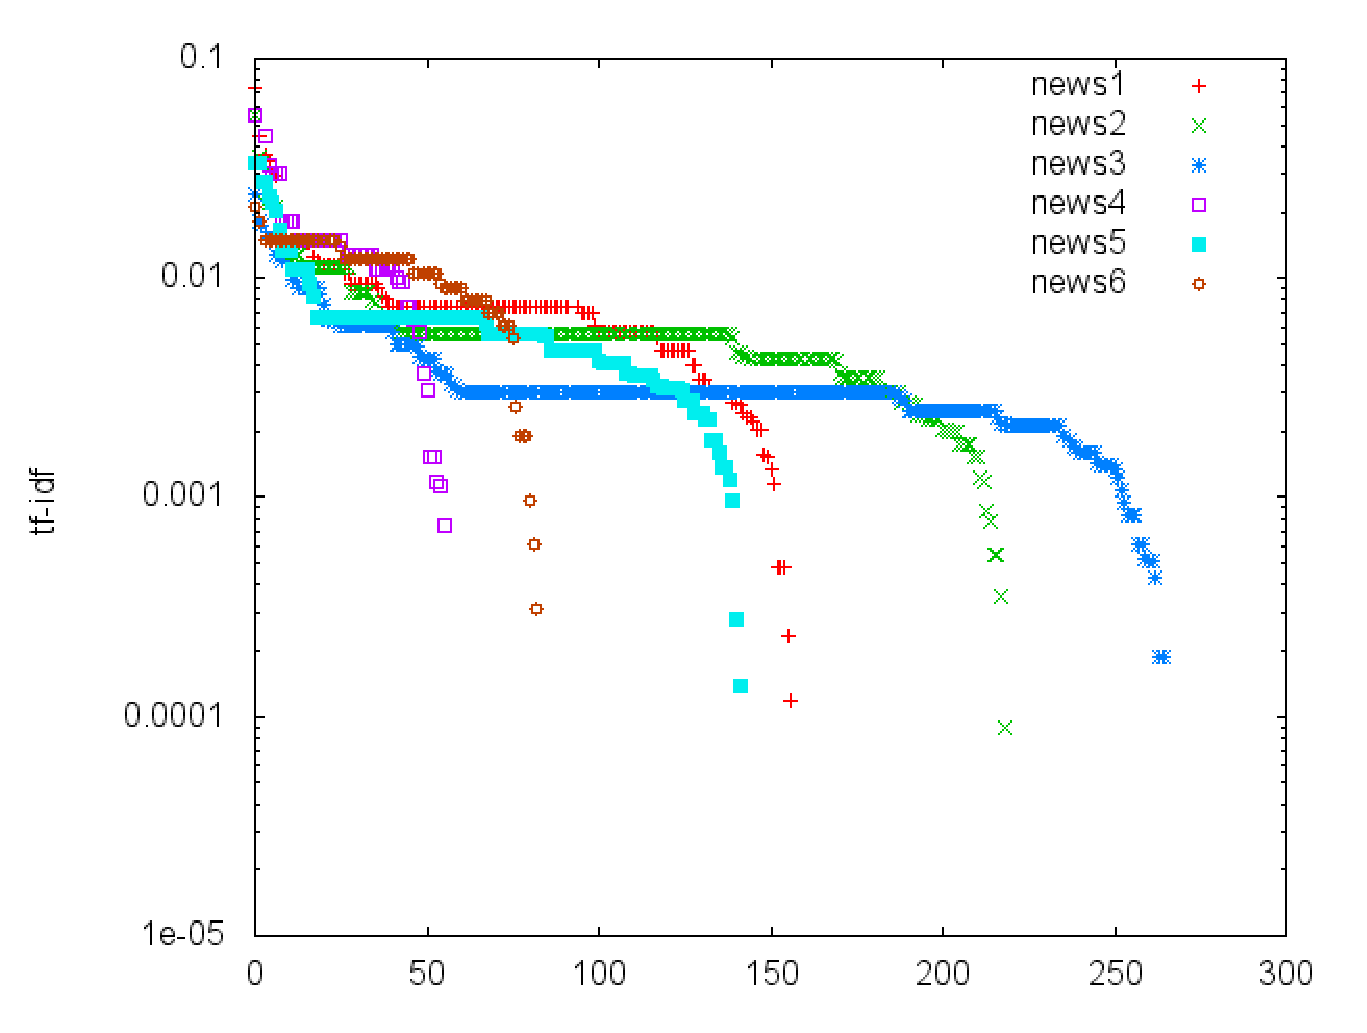
\includegraphics[scale = 0.5]{image/content_word.eps}
  \end{center}
  \caption{tf-idfの計算結果}
  \label{fig2}
\end{figure}

図\ref{fig2}のように、tf-idfの分布が三つの集団に分かれる結果となった。一つは、一番左側のtf-idfが極端に高い単語群である。これは、いわゆるキーワードであると言える。実際、コーヒーの健康への影響を題材にした記事では、「コーヒー」「杯」といった単語がこの集団に属していた。二つ目は、中央部の平らな、平均的なtf-idfをもつ集団である。コーヒーを題材にした記事では、「カフェイン」や「サウスカロライナ」などの内容語が多く所属していたのに対し、「ただし」「よう」等のあまり情報を含まない単語も所属していることが確認された。三つ目は、右側で急降下している、低いtf-idfをもつ集団である。この集団には「て」「に」「を」「は」などの助詞を含む機能語が多く所属していた。

\subsubsection{アラインメント}
「コーヒーの健康に対する影響」のニュースに対して手動で正解を作り、アラインメントの結果からprecision, recall, f-scoreを算出した結果を図\ref{fig3}に示す。
\begin{figure}[htbp]
  \begin{center}
    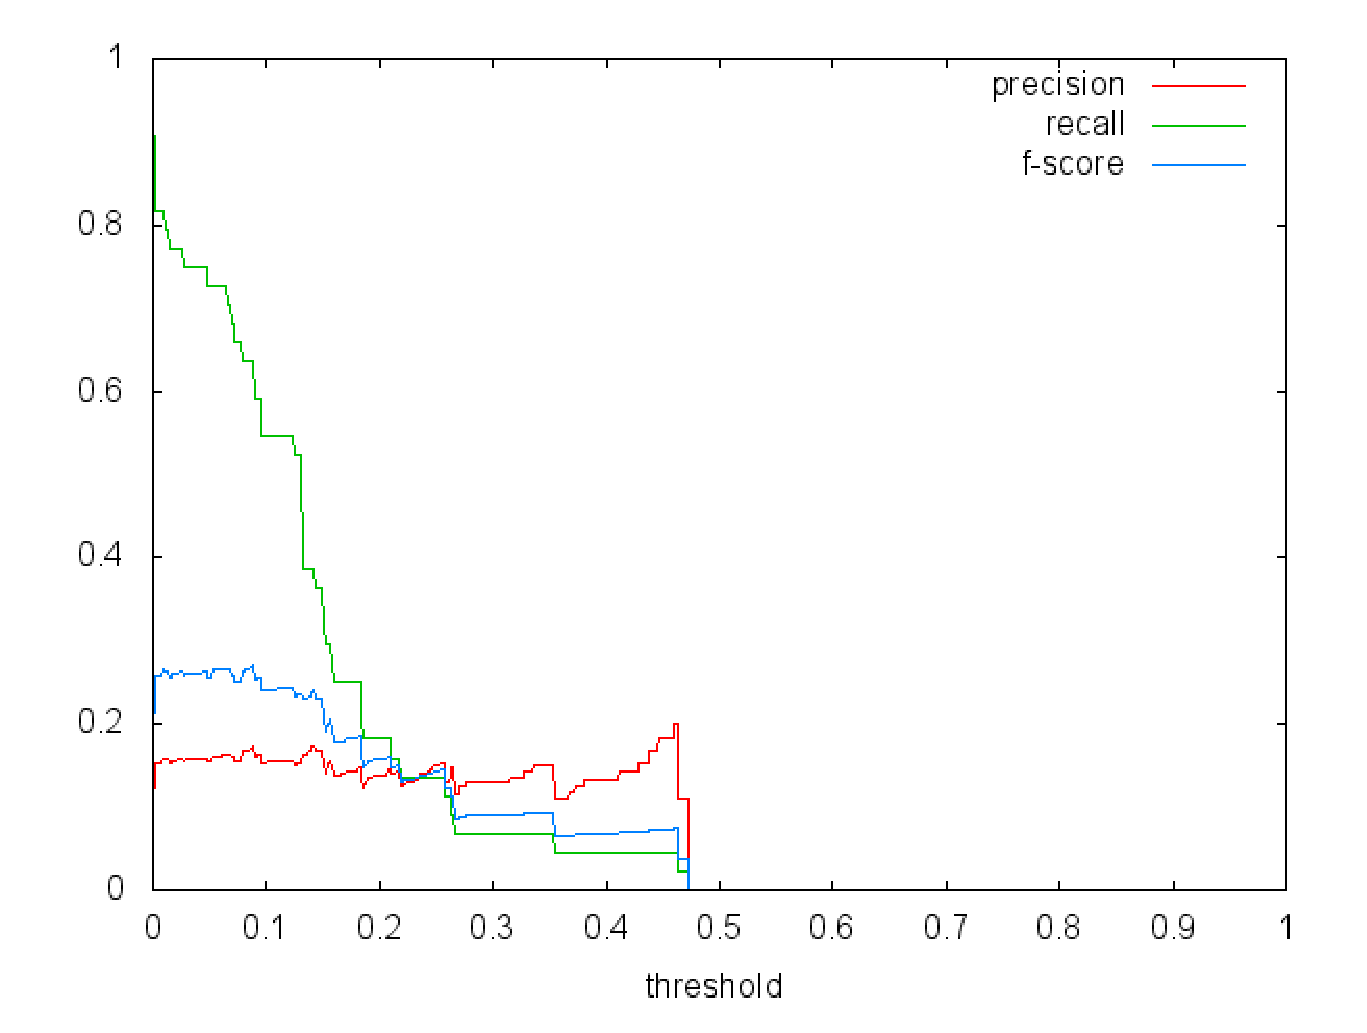
\includegraphics[scale=0.5]{image/score.eps}
  \end{center}
  \caption{アラインメントの結果}
  \label{fig3}
\end{figure}

F値の最大は、閾値が0.088で0.27となった。
本来、閾値が高くなるとrecallは低くなり、precisionが高くなるはずである。しかし、閾値が高くなってもprecisionは低いままであった。また、記事中のほとんど全てのセンテンスと対応づけられてしまうようなtweetが多く見られた。

\section{考察}
\subsection{内容語の抽出}
内容語の抽出では、図\ref{fig2}のように値がおおまかに3つの部分に分かれる結果となった。このうち一番tf-idfの低い集団が、格助詞等の意味を持たない単語の集団であることが確認された。この部分に含まれる単語を除外することで内容語の抽出を行うことができる。しかし、この集団と内容語を含む中央部の集団との境界となるtf-idfの値は一定ではなく、分析する文章により異なる。そこで、それぞれの記事の分布からこの境界の値を算出するアルゴリズムを考える必要がある。また、中央部の集団にも意味を持たない機能語が混ざっているので、それをどのように処理するかを考える必要もある。一つの対策として、現在idfの算出に使用している記事の数が20と少ないので、収集するデータ数を増やしてidfの精度を上げることが考えられる。

\subsection{アラインメント}
アラインメントでは、本来、閾値が高くなるとrecallは低くなり、precisionが高くなるはずであるところ、閾値が高くなってもprecisionは低いままであった。これは、比較的厳選したtweetとnewsの対応でも適合度が低いということで、まだアラインメントの精度が低いことを表す。これはこの先、類似語や関連語の検出を組み込むことで改善されることが期待される。また、記事中のほとんど全てのセンテンスと対応づけられてしまうようなtweetが多く見られたが、そのようなtweetの対応づけはユーザーからみて不適切に見える可能性が高いので、関連語・類似語の検出を組み込んだ後にもそのような問題が起こっていないか注意する必要がある。。

\section{今後の課題}
\subsection{データ収集の自動化}
今後の課題として、内容語の抽出の精度をあげるために、idfの精度を上げることが挙げられる。そのためにはidf算出のためのサンプルデータを増やす必要がある。現在サンプルデータは手動で収集しているが、これでは限界がある上、ニュースの本文では時代が変わると語彙が代わり、idfがうまく機能しない可能性もある。そこで、idf算出のためのサンプルデータ収集を自動化する必要がある。手法としては、現在Twitter社がtweetの検索APIを提供しているので、"@Google\_News\_JP"のようなニュース配信アカウントからインターネット上のニュース記事のURLを自動取得し、そのURLのウェブページからテキストデータを収集する、というものが考えられる。

同様に、アノテーションをする際にそのニュース記事に言及しているtweetを取得することも自動化する必要がある。

\subsection{内容語の抽出}
今回得られた実験結果をもとに、tf-idf分布における下位集団の自動除外を行い、内容語の抽出を行う。また、データ集種の自動化によりidfの精度向上が実現した際には、rf-idf分布における平均的集団から機能語を除去する手段についても検討する。

\subsection{言い換え語・類似語の検出}
今回の実験では未実現となった「言い換えの関係にある語」「互いに類似する語」の検出を実装する必要がある。言い換えの関係にある語はWordNetのSynsetを利用して検出する。これは容易に実現可能であると考えられる。問題は互いに類似する語の検出であるが、Dekang Linの手法\cite{DekangLin}、Latent Spaceでのモデル化\cite{LatentSpace}を実装し、結果を比較検討しながら二つの手法から選択及び組み合わせをして実現する。

\subsection{ユーザー評価の実施}
上記の課題を解決した後に、実際にWebアプリケーションとして本ツールを実装し、ユーザー評価を行う。ユーザー評価では、10ほどの記事にアノテーションを施したものをユーザーに評価してもらい、アノテーションは正確であったか、不要なアノテーションはあったか、このツールによりニュース記事は読みやすくなったかなどをアンケートにより調査する。

\section{結論}
本研究では、ソーシャルネットワーキングサービスであるTwitter上の投稿をインターネット上のニュース記事に自動付与するソーシャルアノテーションツールの構築を行う。要素技術として内容語の抽出、言い換え語の検出、類似語の検出と、それらを利用した短文同士のアラインメントが挙げられる。現段階ではこのうち、内容語の抽出と、言い換え語・類似語を利用しないアラインメントの実装を行った。内容語の抽出に関しては今回得られた結果から良いアルゴリズムを作成する目処を立てる事ができた。アラインメントに関してはまだ精度向上の必要性があるが、実験を通して精度向上のための方針を得ることができた。また、今後の研究で内容語の抽出と言い換え語・類似語の検出を実現することができれば、より高いアラインメント精度の実現が見込めると考える。

ソーシャルアノテーションツールは、情報のプロの書き手と一般人の読み手の距離を縮め、また、難解な情報へのアクセスをより容易にする画期的なツールである。本研究を通して、人の情報との関わり方をより豊かにできるものと自負している。そのために、今後も研究活動により一層尽力して行きたい所存である。

\newpage
\pagestyle{empty}
\begin{thebibliography}{9}
  \bibitem {nlpml} 高村大地, 奥村学.言語処理のための機械学習入門(コロナ社), 2010
  \bibitem {tfidf} Gerard Salton. Introduction to Modern Information Retrieval (Mcgraw Hill, Inc.), 1986
  \bibitem {DekangLin} Dekang Lin. Automatic Retrieval and Clustering of Similar Words. COLING '98 Proceedings of the 17th international conference on Computational linguistics - Volume 2 Pages 768-774
  \bibitem {LatentSpace} Weiwei Guo, Mona Diab. Modeling Sentences in the Latent Space. ACL '12 Proceedings of the 50th Annual Meeting of the Association for Computational Linguistics: Long Papers - Volume 1
Pages 864-872
  \bibitem {CoClustering} Inderjit S Dhilon, Subramanyam Mallela, Dharmendra S. Modha. Information-Theoretic Co-clustering. KDD '03 Proceedings of the ninth ACM SIGKDD international conference on Knowledge discovery and data mining
Pages 89-98
 \bibitem {MeCab} 工藤 拓, 山本 薫, 松本 裕治. Applying Conditional Random Fields to Japanese Morphologiaical Analysis, 情報処理学会研究報告. 自然言語処理研究会報告 2004, Pages 89-96
 \bibitem {information} Christopher D. Manning, Prabhakar Raghavan and Hinrich Schu"tze: Introduction to Information Retrieval, Cambridge University Press, 2008.
\end{thebibliography}
\end{document}

